\documentclass[../main.tex]{subfiles}
\graphicspath{{\subfix{../images/}}}
\begin{document}
\section{Shuffle de \'arboles (Naipear, Barajear o mezclar?)}
En esta seci\'on describiremos el producto tensorial $\Omega[S]\otimes\Omega[T]$ para todo par de \'arboles $S$ y $T$ de $\Omega$. Para ello deberemos introducir la noci\'on del conjunto de shuffles de $S$ y $T$, que ser\'a una gran ayuda para encontrar el producto tensorial. As\'i podremos entender que es el producto tensorial de conjuntos dendroidales.
\subsection{Producto tensorial de \'arboles lineales}
Antes de ver el producto tensorial para \'arboles en general, estudiaremos el caso de \'arboles lineales ya que resulta una tarea m\'as sencilla y la podemos relacionar con el producto cartesiano de conjuntos simpliciales.

Sean $S=L_n$ y $T=L_m$ dos \'arboles lineales, entonces por la proposici\'on 3.30(i),
$$
    \Omega[L_n]\otimes\Omega[L_m]=i_!(\Delta[n])\otimes i_!(\Delta[m])\cong i_!(\Delta[n]\times\Delta[m])
$$
Los simplices no degenerados del producto de dos representables en conjuntos simpliciales son computados mediante un \emph{shuffle}. Un \emph{(n,m)-shuffle} es un camino de longitud m\'axima en el conjunto de orden parcial $[n]\times[m]$.
Los $(n+m)$-simplices no degenerados de $\Delta[n]\times\Delta[m]$ corresponde a los $(n,\text{ }m)$-shuffles. De hecho,
$$
    \Delta[n]\times\Delta[m] = \bigcup_{(n,m)}\Delta[n+m]
$$
Donde la uni\'on recorre todos los posibles $(n,m)$-shuffles.
\begin{ex}
    Sean $n=2$ y $m=1$. Existen tres (2, 1)-shuffles en $[2]\times[1]$, (00,01,02,12), (00,01,11,12) y (00,10,11,12). Tenemos la siguiente figura que representa $\Delta[2]\times\Delta[1]$
    $$
        \xy
        <0.08cm, 0cm>:
        (2.0, 0.0)*{}="1"; %01
        (2.0, 15.0)*{}="2"; %11
        (15.0, 30.0)*{}="3"; %12
        (15.0, 15.0)*{}="4"; %02
        (-20.0, 15.0)*{}="5"; %10
        (-20.0, 0.0)*{}="6"; %00
        "1";"2" **\dir{-};
        "2";"3" **\dir{-};
        "3";"4" **\dir{-};
        "4";"1" **\dir{-};
        "1";"6" **\dir{-};
        "5";"6" **\dir{-};
        "3";"5" **\dir{-};
        "5";"2" **\dir{-};
        "6";"4" **\dir{.};
        (6.0, 0.0)*=0{\scriptstyle 01};
        (6.0, 15.0)*=0{\scriptstyle 11};
        (19.0, 30.0)*=0{\scriptstyle 12};
        (19.0, 15.0)*=0{\scriptstyle 02};
        (-24.0, 15.0)*=0{\scriptstyle 10};
        (-24.0, 0.0)*=0{\scriptstyle 00};
        \endxy
    $$
    Podemos ver que cada (2, 1)-shuffle corresponde a un tetraedro, y hacen una descomposici\'on de $\Delta[2]\times\Delta[1]$ como la uni\'on de tres copias de $\Delta[3]$:
    $$
        \xy<0.08cm, 0cm>:
        (-50,0)*{
                \xy
                <0.08cm, 0cm>:
                (2.0, 0.0)*{}="1"; %01
                (15.0, 30.0)*{}="3"; %12
                (15.0, 15.0)*{}="4"; %02
                (-20.0, 0.0)*{}="6"; %00
                "3";"4" **\dir{-};
                "4";"1" **\dir{-};
                "1";"6" **\dir{-};
                "6";"4" **\dir{.};
                "3";"6" **\dir{-};
                "3";"1" **\dir{-};
                (-3,-5)*{\text{(00, 01, 02, 12)}}
                \endxy
            };
        (0,0)*{
                \xy
                <0.08cm, 0cm>:
                (2.0, 0.0)*{}="1"; %01
                (2.0, 15.0)*{}="2"; %11
                (15.0, 30.0)*{}="3"; %12
                (-20.0, 0.0)*{}="6"; %00
                "1";"2" **\dir{-};
                "2";"3" **\dir{-};
                "1";"6" **\dir{-};
                "3";"6" **\dir{-};
                "2";"6" **\dir{-};
                "3";"1" **\dir{-};
                (-3,-5)*{\text{(00, 01, 11, 12)}}
                \endxy
            };
        (50,0)*{
                \xy
                <0.08cm, 0cm>:
                (2.0, 15.0)*{}="2"; %11
                (15.0, 30.0)*{}="3"; %12
                (-20.0, 15.0)*{}="5"; %10
                (-20.0, 0.0)*{}="6"; %00
                "2";"3" **\dir{-};
                "5";"6" **\dir{-};
                "3";"5" **\dir{-};
                "5";"2" **\dir{-};
                "5";"2" **\dir{-};
                "6";"2" **\dir{-};
                "6";"3" **\dir{.};
                (-3,-5)*{\text{(00, 10, 11, 12)}}
                \endxy
            };
        \endxy
    $$
\end{ex}
\subsection{Producto tensorial de \'arboles}
\subsubsection{Shuffles y conjuntos de shuffles}
En este apartado vamos a introducir la noci\'on de un shuffle entre dos \'arboles y la coleci\'on de todos ellos. Tambi\'en daremos ejemplos extensos de como calcular dichos shuffles.

\begin{defi}
    Sea $S$ y $T$ dos objetos de $\Omega$. Un \emph{shuffle} de $S$ y $T$ es un \'arbol $R$ cuyo conjunto de aristas es un subconjunto de $E(S)\times E(T)$. La ra\'iz de $R$ es $(a,\text{ }x)$, donde $a$ es la ra\'iz de $S$ y $x$ es la ra\'iz de $T$,
    y sus hojas son todos los pares $(l_S,\text{ }l_T)$, donde $l_S$ es una hoja de $S$ y $l_T$ es una hoja de $T$. Los v\'ertices son de la forma
    $$
        \xy
        <0.08cm, 0cm>:
        %Vertices%
        (0.0, 0.0)*{}="1"; %root_b-x
        (0.0, 10.0)*\cir<2pt>{}="2"; %uW
        (-7.5, 20.0)*{}="3"; %leaf_a_1-x
        (7.5, 20.0)*{}="4"; %leaf_a_n-x
        %Edges%
        "1";"2" **\dir{-};
        "2";"3" **\dir{-};
        "2";"4" **\dir{-};
        %Labels%
        (3.0, 10.0)*=0{\scriptstyle u};
        (-5.5, 5)*=0{\scriptstyle (b,\text{ }x)};
        (-10, 13.0)*=0{\scriptstyle (a_1,\text{ }x)};
        (10, 13.0)*=0{\scriptstyle (a_n,\text{ }x)};
        (0,15)*{\dots};
        \endxy
        \xy
        <0.08cm, 0cm>:
        (-15, 0.0)*{}="1";
        (15, 10.0)*{}="2";
        (0,10)*{\rm o};
        \endxy
        \xy
        <0.08cm, 0cm>:
        %Vertices%
        (0.0, 0.0)*{}="1"; %root_a-y
        (0.0, 10.0)*=0{\bullet}="2"; %vB
        (-7.5, 20.0)*{}="3"; %leaf_a-x_1
        (7.5, 20.0)*{}="4"; %leaf_a-x_m
        %Edges%
        "1";"2" **\dir{-};
        "2";"3" **\dir{-};
        "2";"4" **\dir{-};
        %Labels%
        (3.0, 10.0)*=0{\scriptstyle v};
        (-5.5, 5)*=0{\scriptstyle (a,\text{ }y)};
        (-10, 13.0)*=0{\scriptstyle (a,\text{ }x_1)};
        (10, 13.0)*=0{\scriptstyle (a,\text{ }x_m)};
        (0,15)*{\dots};
        \endxy
    $$
    Donde $u$ es un v\'ertice de $S$ con entradas $a_1,\dots,a_n$ y salida $b$, y $v$ es un v\'ertice de $T$ con entradas $x_1,\dots,x_m$ y salida $y$. Nos referiremos a los dos tipos de v\'ertices como \emph{v\'ertices blancos} y \emph{v\'ertices negres}, respectivamente. Para diferenciarlos visualmente los pintaremos con $\circ$ y $\bullet$, respectivamente.

    Observamos que existe una biyecci\'on entre los shuffles de dos \'arboles lineales $L_n$ y $L_m$ con los $(n,\text{ }m)$-shuffles de $[n]\times[m]$.
\end{defi}

\begin{defi}
    Sean $S$ y $T$ dos \'arboles. El \emph{conjunto de shuffles de $S$ y $T$} es la colecci\'on de todos los shuffles posibles entre $S$ y $T$. La cardinalidad de este conjunto la denotaremos por $sh(S,\text{ }T)$.
\end{defi}
\begin{prop}
    El n\'umero de shuffles $sh(S,\text{ }T)$ de dos \'arboles $S$ y $T$ satisface tres propiedades:
    \begin{enumerate}
        \item[{\rm (i)}] $sh(S, \text{ }T) = sh(T, \text{ }S)$
        \item[{\rm (ii)}] Si $T$ es un \'arbol unitario $\eta$, entonces $sh(S, \text{ }\eta)=1$
        \item[{\rm (iii)}] Si $S=C_n[S_1,\dots,S_n]$ y $T=C_m[T_1,\dots,T_m]$, entonces
              $$
                  sh(S, \text{ }T)  = \prod_{i=1}^n sh(S_i, \text{ }T) + \prod_{j=1}^m sh(S, \text{ }T_j)
              $$
    \end{enumerate}
    Donde $C_n$ y $C_m$ son $n$ y $m$-corolas, respectivamente; y $C_n[S_1,\dots,S_n]$ es una $n$-corola que cada hoja $i$-esima la conectamos con la ra\'iz del \'arbol $S_i$.
\end{prop}
\begin{ex}
    Sean $S$ y $T$ los \'arboles
    $$
        \xy
        <0.08cm, 0cm>:
        %Vertices%
        (0.0, 0.0)*{}="1"; %root_a
        (0.0, 10.0)*\cir<2pt>{}="2"; %0W
        (-15.0, 20.0)*{}="3"; %leaf_b
        (15.0, 20.0)*\cir<2pt>{}="7"; %1W
        (5.0, 30.0)*{}="8"; %leaf_d
        (15.0, 30.0)*{}="9"; %leaf_e
        (25.0, 30.0)*{}="10"; %leaf_f
        %Edges%
        "1";"2" **\dir{-};
        "2";"3" **\dir{-};
        "2";"7" **\dir{-};
        "7";"8" **\dir{-};
        "7";"9" **\dir{-};
        "7";"10" **\dir{-};
        %Labels%
        (-2.0, 5.0)*=0{\scriptstyle a};
        (-11, 15.0)*=0{\scriptstyle b};
        (10.5, 15.0)*=0{\scriptstyle c};
        (7.0, 25.0)*=0{\scriptstyle d};
        (13.0, 25.0)*=0{\scriptstyle e};
        (22.5, 25.0)*=0{\scriptstyle f};
        (-13,0)*{S};
        \endxy
        \xy
        <0.08cm, 0cm>:
        (-10, 0.0)*{}="1";
        (10, 10.0)*{}="2";
        \endxy
        \xy
        <0.08cm, 0cm>:
        %Vertices%
        (0.0, 0.0)*{}="1"; %root_x
        (0.0, 10.0)*=0{\bullet}="2"; %0B
        (0.0, 20.0)*{}="3"; %leaf_y
        %Edges%
        "1";"2" **\dir{-};
        "2";"3" **\dir{-};
        %Labels%
        (-2.0, 5.0)*=0{\scriptstyle x};
        (-2.0, 15.0)*=0{\scriptstyle y};
        (-13,0)*{T};
        \endxy
    $$
    El conjunto de shuffles de $S$ y $T$ consiste de los siguientes tres \'arboles:
    \begin{equation}
        \xy
        <0.08cm, 0cm>:
        %Vertices%
        (0.0, 0.0)*{}="1"; %root_a-x
        (0.0, 12.5)*\cir<2pt>{}="2"; %0W
        (-16.0, 25.0)*=0{\bullet}="3"; %2B
        (-16.0, 37.5)*{}="4"; %leaf_b-y
        (16.0, 25.0)*\cir<2pt>{}="5"; %1W
        (0.0, 37.5)*=0{\bullet}="6"; %2B
        (0.0, 50.0)*{}="7"; %leaf_d-y
        (16.0, 37.5)*=0{\bullet}="8"; %2B
        (16.0, 50.0)*{}="9"; %leaf_e-y
        (32.0, 37.5)*=0{\bullet}="10"; %2B
        (32.0, 50.0)*{}="11"; %leaf_f-y
        %Edges%
        "1";"2" **\dir{-};
        "2";"3" **\dir{-};
        "3";"4" **\dir{-};
        "2";"5" **\dir{-};
        "5";"6" **\dir{-};
        "6";"7" **\dir{-};
        "5";"8" **\dir{-};
        "8";"9" **\dir{-};
        "5";"10" **\dir{-};
        "10";"11" **\dir{-};
        %Labels%
        (-5, 6.25)*=0{\scriptstyle (a,\text{ }x)};
        (-15, 18.75)*=0{\scriptstyle (b,\text{ }x)};
        (-21.0, 31.25)*=0{\scriptstyle (b,\text{ }y)};
        (15.0, 18.75)*=0{\scriptstyle (c,\text{ }x)};
        (1.0, 31.25)*=0{\scriptstyle (d,\text{ }x)};
        (-5, 43.75)*=0{\scriptstyle (d,\text{ }y)};
        (16.0, 31.25)*=0{\scriptstyle (e,\text{ }x)};
        (16.0, 43.75)*=0{\scriptstyle (e,\text{ }y)};
        (31.0, 31.25)*=0{\scriptstyle (f,\text{ }x)};
        (37, 43.75)*=0{\scriptstyle (f,\text{ }y)};
        (-13,0)*{R_1};
        \endxy
        \xy
        <0.08cm, 0cm>:
        (-10, 0.0)*{}="1";
        (10, 10.0)*{}="2";
        \endxy
        \xy
        <0.08cm, 0cm>:
        %Vertices%
        (0.0, 0.0)*{}="1"; %root_a-x
        (0.0, 12.5)*\cir<2pt>{}="2"; %0W
        (-8.0, 25.0)*=0{\bullet}="3"; %2B
        (-8.0, 37.5)*{}="4"; %leaf_b-y
        (8.0, 25.0)*=0{\bullet}="5"; %2B
        (8.0, 37.5)*\cir<2pt>{}="6"; %1W
        (-8.0, 50.0)*{}="7"; %leaf_d-y
        (8.0, 50.0)*{}="8"; %leaf_e-y
        (24.0, 50.0)*{}="9"; %leaf_f-y
        %Edges%
        "1";"2" **\dir{-};
        "2";"3" **\dir{-};
        "3";"4" **\dir{-};
        "2";"5" **\dir{-};
        "5";"6" **\dir{-};
        "6";"7" **\dir{-};
        "6";"8" **\dir{-};
        "6";"9" **\dir{-};
        %Labels%
        (-5.0, 6.25)*=0{\scriptstyle (a,\text{ }x)};
        (-9.5, 18.75)*=0{\scriptstyle (b,\text{ }x)};
        (-13, 31.25)*=0{\scriptstyle (b,\text{ }y)};
        (9.5, 18.75)*=0{\scriptstyle (c,\text{ }x)};
        (13.0, 31.25)*=0{\scriptstyle (c,\text{ }y)};
        (-7, 43.75)*=0{\scriptstyle (d,\text{ }y)};
        (8, 43.75)*=0{\scriptstyle (e,\text{ }y)};
        (23.0, 43.75)*=0{\scriptstyle (f,\text{ }y)};
        (-13,0)*{R_2};
        \endxy
        \xy
        <0.08cm, 0cm>:
        (-10, 0.0)*{}="1";
        (10, 10.0)*{}="2";
        \endxy
        \xy
        <0.08cm, 0cm>:
        %Vertices%
        (0.0, 0.0)*{}="1"; %root_a-x
        (0.0, 12.5)*=0{\bullet}="2"; %2B
        (0.0, 25.0)*\cir<2pt>{}="3"; %0W
        (-8.0, 37.5)*{}="4"; %leaf_b-y
        (8.0, 37.5)*\cir<2pt>{}="5"; %1W
        (-8.0, 50.0)*{}="6"; %leaf_d-y
        (8.0, 50.0)*{}="7"; %leaf_e-y
        (24.0, 50.0)*{}="8"; %leaf_f-y
        %Edges%
        "1";"2" **\dir{-};
        "2";"3" **\dir{-};
        "3";"4" **\dir{-};
        "3";"5" **\dir{-};
        "5";"6" **\dir{-};
        "5";"7" **\dir{-};
        "5";"8" **\dir{-};
        %Labels%
        (-5.0, 6.25)*=0{\scriptstyle (a,\text{ }x)};
        (-5.0, 18.75)*=0{\scriptstyle (a,\text{ }y)};
        (-9.5, 31.25)*=0{\scriptstyle (b,\text{ }y)};
        (9.5, 31.25)*=0{\scriptstyle (c,\text{ }y)};
        (-7, 43.75)*=0{\scriptstyle (d,\text{ }y)};
        (8.0, 43.75)*=0{\scriptstyle (e,\text{ }y)};
        (23, 43.75)*=0{\scriptstyle (f,\text{ }y)};
        (-13,0)*{R_3};
        \endxy
    \end{equation}
\end{ex}

El conjunto de shuffles de $S$ y $T$ es \emph{ordenado parcialmente}. El \'arbol minimal $R_1$ en el conjunto ordenado parcialmente se obtiene mediante la inserci\'on de una copia del \'arbol negro $T$ en cada entrada del \'arbol blanco $S$.
Es decir, primero hacemos una copia del \'arbol $S$ de la forma $S\otimes r_T$, donde todas sus aristas han sido renombradas como $(\underline{\hspace{.25cm}},\text{ }r_T)$, siendo $r_T$ la ra\'iz del \'arbol $T$.
Luego hacemos una copia del \'arbol $T$ de la forma $l\otimes T$, para toda hoja $l$ de $S$; donde todas sus aristas han sido renombradas como $(l,\text{ }\underline{\hspace{.25cm}})$.
Finalmente, obtenemos el \'arbol $R_1$ encajando las \'ultimas copias encima de las hojas de la forma $(l,\text{ }r_T)$ de la primera copia.
El \'arbol maximal $R_N$ en el conjunto ordenado parcialmente se obtiene mediante la inserci\'on de una copia del \'arbol blanco $S$ en cada entrada del \'arbol negro $T$.
Los \'arboles $R_1$ y $R_n$ deber\'ian lucir de la siguiente manera

$$
    \xy<0.1cm, 0cm>:
    (0,0)*=0{}="1";
    (0,10)*=0{}="2";
    (-0,20)*=0{}="a";
    (-5,20)*=0{}="3";
    (5,20)*=0{}="4";
    (-20,30)*=0{}="5";
    (20,30)*=0{}="6";
    (0,30)*=0{}="b";
    (0,16)*=0{S};
    "1";"2" **\dir{-};
    "2";"3" **\dir{-};
    "2";"4" **\dir{-};
    "3";"4" **\dir{-};
    "3";"5" **\dir{-};
    "4";"6" **\dir{-};
    "a";"b" **\dir{-};
    (-25,35)*=0{}="9";
    (-15,35)*=0{}="10";
    (-5,35)*=0{}="11";
    (5,35)*=0{}="12";
    (15,35)*=0{}="15";
    (25,35)*=0{}="16";
    "5";"9" **\dir{-};
    "5";"10" **\dir{-};
    "9";"10" **\dir{-};
    "b";"11" **\dir{-};
    "b";"12" **\dir{-};
    "11";"12" **\dir{-};
    "6";"15" **\dir{-};
    "6";"16" **\dir{-};
    "15";"16" **\dir{-};
    (-20,33)*=0{T};
    (0,33)*=0{T};
    (20,33)*=0{T};
    (-10,0)*=0{R_1};
    \endxy
    \qquad
    \qquad
    \xy<0.1cm, 0cm>:
    (0,0)*=0{}="1";
    (0,10)*=0{}="2";
    (-2.5,20)*=0{}="a";
    (2.5,20)*=0{}="b";
    (-5,20)*=0{}="3";
    (5,20)*=0{}="4";
    (-20,30)*=0{}="5";
    (20,30)*=0{}="6";
    (-5,30)*=0{}="c";
    (5,30)*=0{}="d";
    (0,16)*=0{T};
    "1";"2" **\dir{-};
    "2";"3" **\dir{-};
    "2";"4" **\dir{-};
    "3";"4" **\dir{-};
    "3";"5" **\dir{-};
    "4";"6" **\dir{-};
    "a";"c" **\dir{-};
    "b";"d" **\dir{-};
    (-25,35)*=0{}="9";
    (-15,35)*=0{}="10";
    (-10,35)*=0{}="11";
    (-2,35)*=0{}="12";
    (2,35)*=0{}="13";
    (10,35)*=0{}="14";
    (15,35)*=0{}="15";
    (25,35)*=0{}="16";
    "5";"9" **\dir{-};
    "5";"10" **\dir{-};
    "9";"10" **\dir{-};
    "c";"11" **\dir{-};
    "c";"12" **\dir{-};
    "11";"12" **\dir{-};
    "d";"13" **\dir{-};
    "d";"14" **\dir{-};
    "13";"14" **\dir{-};
    "6";"15" **\dir{-};
    "6";"16" **\dir{-};
    "15";"16" **\dir{-};
    (-20,33)*=0{S};
    (-5.5,33)*=0{S};
    (5.5,33)*=0{S};
    (20,33)*=0{S};
    (-10,0)*=0{R_N};
    \endxy
$$
Existen los \emph{shuffles intermediarios} $R_k$ $(1 < k < N)$ entre $R_1$ y $R_N$ obtenidos filtrando los v\'ertices negros en $R_1$ hacia la ra\'iz del \'arbol mediante intercambios con los v\'ertices blancos.
Todo $R_k$ se obtiene desde un $R_l$ anterior. Es decir, cada intercambio se basa en transformar una configuraci\'on de $R_l$
\begin{equation}
    \xy
    <0.08cm, 0cm>:
    %Vertices%
    (0.0, 0.0)*{}="1"; %root_a-x
    (0.0, 15.0)*\cir<2pt>{}="2"; %0W
    (-25.0, 30.0)*=0{\bullet}="3"; %1B
    (-37.5, 45.0)*{}="4"; %leaf_b_1-y_1
    (-12.5, 45.0)*{}="5"; %leaf_b_n-y_1
    (25.0, 30.0)*=0{\bullet}="6"; %2B
    (12.5, 45.0)*{}="7"; %leaf_b_1-y_m
    (37.5, 45.0)*{}="8"; %leaf_b_n-y_m
    %Edges%
    "1";"2" **\dir{-};
    "2";"3" **\dir{-};
    "3";"4" **\dir{-};
    "3";"5" **\dir{-};
    "2";"6" **\dir{-};
    "6";"7" **\dir{-};
    "6";"8" **\dir{-};
    %Labels%
    (-5.5, 7.5)*=0{\scriptstyle (a,\text{ }x)};
    (-19.5, 21)*=0{\scriptstyle (a,\text{ }y_1)};
    (-39, 37.5)*=0{\scriptstyle (b_1,\text{ }y_1)};
    (-11, 37.5)*=0{\scriptstyle (b_n,\text{ }y_1)};
    (19.5, 21)*=0{\scriptstyle (a,\text{ }y_m)};
    (10.5, 37.5)*=0{\scriptstyle (b_1,\text{ }y_m)};
    (39.5, 37.5)*=0{\scriptstyle (b_n,\text{ }y_m)};
    (-25,35)*{\dots};
    (25,35)*{\dots};
    (0,20)*{\dots\dots};
    \endxy
\end{equation}
A una configuraci\'on de $R_k$
\begin{equation}
    \xy
    <0.08cm, 0cm>:
    %Vertices%
    (0.0, 0.0)*{}="1"; %root_a-x
    (0.0, 15.0)*=0{\bullet}="2"; %0B
    (-25.0, 30.0)*\cir<2pt>{}="3"; %1W
    (-37.5, 45.0)*{}="4"; %leaf_b_1-y_1
    (-12.5, 45.0)*{}="5"; %leaf_b_1-y_m
    (25.0, 30.0)*\cir<2pt>{}="6"; %2W
    (12.5, 45.0)*{}="7"; %leaf_b_n-y_1
    (37.5, 45.0)*{}="8"; %leaf_b_n-y_m
    %Edges%
    "1";"2" **\dir{-};
    "2";"3" **\dir{-};
    "3";"4" **\dir{-};
    "3";"5" **\dir{-};
    "2";"6" **\dir{-};
    "6";"7" **\dir{-};
    "6";"8" **\dir{-};
    %Labels%
    (-5.5, 7.5)*=0{\scriptstyle (a,\text{ }x)};
    (-19.5, 21)*=0{\scriptstyle (b_1,\text{ }x)};
    (-39, 37.5)*=0{\scriptstyle (b_1,\text{ }y_1)};
    (-11, 37.5)*=0{\scriptstyle (b_1,\text{ }y_m)};
    (19.5, 21)*=0{\scriptstyle (b_n,\text{ }x)};
    (10.5, 37.5)*=0{\scriptstyle (b_n,\text{ }y_1)};
    (39.5, 37.5)*=0{\scriptstyle (b_n,\text{ }y_m)};
    (-25,35)*{\dots};
    (25,35)*{\dots};
    (0,20)*{\dots\dots};
    \endxy
\end{equation}
Si un shuffle $R_k$ se obtiene the otro shuffle $R_l$ mediante la norma de arriba, entonces decimos que $R_k$ se obtiene mediante \emph{un solo intercambio} y lo denotaremos por $R_l\le R_k$.
As\'i, obtenemos un orden parcial en el conjunto de todos los shuffles.

Tenemos que espicificar el caso de un intercambio con un \'arboles sin entradas, es decir, $n=0$ o $m=0$. Si $m=0$ y $n\ne 0$, entonces tenemos el intercambio
\begin{equation}
    \xy
    <0.08cm, 0cm>:
    %Vertices%
    (0.0, 0.0)*{}="1"; %root_a-x
    (0.0, 10.0)*\cir<2pt>{}="2"; %0W
    %Edges%
    "1";"2" **\dir{-};
    %Labels%
    (-5.0, 5.0)*=0{\scriptstyle (a,\text{ }x)};
    \endxy
    \xy
    <0.08cm, 0cm>:
    (-20, 0.0)*{}="1";
    (20, 10.0)*{}="2";
    {\ar(-10, 10)*{};(10,10)*{}};
    \endxy
    \xy
    <0.08cm, 0cm>:
    %Vertices%
    (0.0, 0.0)*{}="1"; %root_a-x
    (0.0, 10.0)*=0{\bullet}="2"; %0B
    (-12.5, 20.0)*\cir<2pt>{}="3"; %1W
    (12.5, 20.0)*\cir<2pt>{}="4"; %2W
    %Edges%
    "1";"2" **\dir{-};
    "2";"3" **\dir{-};
    "2";"4" **\dir{-};
    %Labels%
    (-5.0, 5.0)*=0{\scriptstyle (a,\text{ }x)};
    (-14, 15.0)*=0{\scriptstyle (b_1,\text{ }x)};
    (14, 15.0)*=0{\scriptstyle (b_n,\text{ }x)};
    (0,13.5)*{\dots};
    \endxy
\end{equation}

Si $n=0$ y $m\ne 0$, entonces tenemos el intercambio
\begin{equation}
    \xy
    <0.08cm, 0cm>:
    %Vertices%
    (0.0, 0.0)*{}="1"; %root_a-x
    (0.0, 10.0)*\cir<2pt>{}="2"; %0W
    (-12.5, 20.0)*=0{\bullet}="3"; %1B
    (12.5, 20.0)*=0{\bullet}="4"; %2B
    %Edges%
    "1";"2" **\dir{-};
    "2";"3" **\dir{-};
    "2";"4" **\dir{-};
    %Labels%
    (-5.0, 5.0)*=0{\scriptstyle (a,\text{ }x)};
    (-14, 15.0)*=0{\scriptstyle (a,\text{ }y_1)};
    (14, 15.0)*=0{\scriptstyle (a,\text{ }y_m)};
    (0,13.5)*{\dots};
    \endxy
    \xy
    <0.08cm, 0cm>:
    (-20, 0.0)*{}="1";
    (20, 10.0)*{}="2";
    {\ar(-10, 10)*{};(10,10)*{}};
    \endxy
    \xy
    <0.08cm, 0cm>:
    %Vertices%
    (0.0, 0.0)*{}="1"; %root_a-x
    (0.0, 10.0)*\cir<2pt>{}="2"; %0W
    %Edges%
    "1";"2" **\dir{-};
    %Labels%
    (-5.0, 5.0)*=0{\scriptstyle (a,\text{ }x)};
    \endxy
\end{equation}

Finalmente, si $n=m=0$, entonces tenemos el intercambio
\begin{equation}
    \xy
    <0.08cm, 0cm>:
    %Vertices%
    (0.0, 0.0)*{}="1"; %root_a-x
    (0.0, 10.0)*\cir<2pt>{}="2"; %0W
    %Edges%
    "1";"2" **\dir{-};
    %Labels%
    (-5.0, 5.0)*=0{\scriptstyle (a,\text{ }x)};
    \endxy
    \xy
    <0.08cm, 0cm>:
    (-20, 0.0)*{}="1";
    (20, 10.0)*{}="2";
    {\ar(-10, 10)*{};(10,10)*{}};
    \endxy
    \xy
    <0.08cm, 0cm>:
    %Vertices%
    (0.0, 0.0)*{}="1"; %root_a-x
    (0.0, 10.0)*=0{\bullet}="2"; %0B
    %Edges%
    "1";"2" **\dir{-};
    %Labels%
    (-5.0, 5.0)*=0{\scriptstyle (a,\text{ }x)};
    \endxy
\end{equation}

\begin{ex}
    Sean $S$ y $T$ los \'arboles
    $$
        \xy
        <0.08cm, 0cm>:
        %Vertices%
        (0.0, 0.0)*{}="1"; %root_0
        (0.0, 10.0)*\cir<2pt>{}="2"; %0W
        (0.0, 20.0)*\cir<2pt>{}="3"; %1W
        (-7.5, 30.0)*{}="4"; %leaf_2
        (7.5, 30.0)*{}="5"; %leaf_3
        %Edges%
        "1";"2" **\dir{-};
        "2";"3" **\dir{-};
        "3";"4" **\dir{-};
        "3";"5" **\dir{-};
        %Labels%
        (-2.0, 5.0)*=0{\scriptstyle 0};
        (-2.0, 15.0)*=0{\scriptstyle 1};
        (-6, 25.0)*=0{\scriptstyle 2};
        (1.5, 25.0)*=0{\scriptstyle 3};
        (-13,0)*{S};
        \endxy
        \xy
        <0.08cm, 0cm>:
        (-20, 0.0)*{}="1";
        (20, 10.0)*{}="2";
        \endxy
        \xy
        <0.08cm, 0cm>:
        %Vertices%
        (0.0, 0.0)*{}="1"; %root_a
        (0.0, 10.0)*=0{\bullet}="2"; %0B
        (-7.5, 20.0)*=0{\bullet}="3"; %1B
        (-7.5, 30.0)*{}="4"; %leaf_c
        (7.5, 20.0)*=0{\bullet}="5"; %2B
        (7.5, 30.0)*{}="6"; %leaf_e
        %Edges%
        "1";"2" **\dir{-};
        "2";"3" **\dir{-};
        "3";"4" **\dir{-};
        "2";"5" **\dir{-};
        "5";"6" **\dir{-};
        %Labels%
        (-2.0, 5.0)*=0{\scriptstyle a};
        (-5.75, 15.0)*=0{\scriptstyle b};
        (-9.5, 25.0)*=0{\scriptstyle c};
        (1.5, 15.0)*=0{\scriptstyle d};
        (5.5, 25.0)*=0{\scriptstyle e};
        (-13,0)*{T};
        \endxy
    $$
    Existen catorce shuffles $R_1,\dots,R_{14}$ de $S$ y $T$. Mostramos una lista completa de ellos. Marcaremos los nombres de las aristas en los tres primeros shuffles.
    $$
        \xy
        <0.08cm, 0cm>:
        %Vertices%
        (0.0, 0.0)*{}="1"; %root_0-a
        (0.0, 10.0)*\cir<2pt>{}="2"; %0W
        (0.0, 20.0)*\cir<2pt>{}="3"; %1W
        (-15.0, 30.0)*=0{\bullet}="4"; %0B
        (-22.5, 40.0)*=0{\bullet}="5"; %1B
        (-22.5, 50.0)*{}="6"; %leaf_2-c
        (-7.5, 40.0)*=0{\bullet}="7"; %2B
        (-7.5, 50.0)*{}="8"; %leaf_2-e
        (15.0, 30.0)*=0{\bullet}="9"; %0B
        (7.5, 40.0)*=0{\bullet}="10"; %1B
        (7.5, 50.0)*{}="11"; %leaf_3-c
        (22.5, 40.0)*=0{\bullet}="12"; %2B
        (22.5, 50.0)*{}="13"; %leaf_3-e
        %Edges%
        "1";"2" **\dir{-};
        "2";"3" **\dir{-};
        "3";"4" **\dir{-};
        "4";"5" **\dir{-};
        "5";"6" **\dir{-};
        "4";"7" **\dir{-};
        "7";"8" **\dir{-};
        "3";"9" **\dir{-};
        "9";"10" **\dir{-};
        "10";"11" **\dir{-};
        "9";"12" **\dir{-};
        "12";"13" **\dir{-};
        %Labels%
        (-5.0, 5.0)*=0{\scriptstyle (0,\text{ }a)};
        (-5.0, 15.0)*=0{\scriptstyle (1,\text{ }a)};
        (-14.5, 25.0)*=0{\scriptstyle (2,\text{ }a)};
        (-24, 35.0)*=0{\scriptstyle (2,\text{ }b)};
        (-27, 45.0)*=0{\scriptstyle (2,\text{ }c)};
        (-6, 35.0)*=0{\scriptstyle (2,\text{ }d)};
        (-12, 45.0)*=0{\scriptstyle (2,\text{ }e)};
        (14.5, 25.0)*=0{\scriptstyle (3,\text{ }a)};
        (6, 35.0)*=0{\scriptstyle (3,\text{ }b)};
        (3, 45.0)*=0{\scriptstyle (3,\text{ }c)};
        (24, 35.0)*=0{\scriptstyle (3,\text{ }d)};
        (18, 45.0)*=0{\scriptstyle (3,\text{ }e)};
        (-13,0)*{R_1};
        \endxy
        \xy
        <0.08cm, 0cm>:
        (-5, 0.0)*{}="1";
        (5, 10.0)*{}="2";
        \endxy
        \xy
        <0.08cm, 0cm>:
        %Vertices%
        (0.0, 0.0)*{}="1"; %root_0-a
        (0.0, 10.0)*\cir<2pt>{}="2"; %0W
        (0.0, 20.0)*=0{\bullet}="3"; %0B
        (-15.0, 30.0)*\cir<2pt>{}="4"; %1W
        (-22.5, 40.0)*=0{\bullet}="5"; %1B
        (-22.5, 50.0)*{}="6"; %leaf_2-c
        (-7.5, 40.0)*=0{\bullet}="7"; %1B
        (-7.5, 50.0)*{}="8"; %leaf_3-c
        (15.0, 30.0)*\cir<2pt>{}="9"; %1W
        (7.5, 40.0)*=0{\bullet}="10"; %2B
        (7.5, 50.0)*{}="11"; %leaf_2-e
        (22.5, 40.0)*=0{\bullet}="12"; %2B
        (22.5, 50.0)*{}="13"; %leaf_3-e
        %Edges%
        "1";"2" **\dir{-};
        "2";"3" **\dir{-};
        "3";"4" **\dir{-};
        "4";"5" **\dir{-};
        "5";"6" **\dir{-};
        "4";"7" **\dir{-};
        "7";"8" **\dir{-};
        "3";"9" **\dir{-};
        "9";"10" **\dir{-};
        "10";"11" **\dir{-};
        "9";"12" **\dir{-};
        "12";"13" **\dir{-};
        %Labels%
        (-5.0, 5.0)*=0{\scriptstyle (0,\text{ }a)};
        (-5.0, 15.0)*=0{\scriptstyle (1,\text{ }a)};
        (-14.5, 25.0)*=0{\scriptstyle (1,\text{ }b)};
        (-24, 35.0)*=0{\scriptstyle (2,\text{ }b)};
        (-27, 45.0)*=0{\scriptstyle (2,\text{ }c)};
        (-6, 35.0)*=0{\scriptstyle (3,\text{ }b)};
        (-12, 45.0)*=0{\scriptstyle (3,\text{ }c)};
        (14.5, 25.0)*=0{\scriptstyle (1,\text{ }d)};
        (6, 35.0)*=0{\scriptstyle (2,\text{ }d)};
        (3, 45.0)*=0{\scriptstyle (2,\text{ }e)};
        (24, 35.0)*=0{\scriptstyle (3,\text{ }d)};
        (18, 45.0)*=0{\scriptstyle (3,\text{ }e)};
        (-13,0)*{R_2};
        \endxy
        \xy
        <0.08cm, 0cm>:
        (-5, 0.0)*{}="1";
        (5, 10.0)*{}="2";
        \endxy
        \xy
        <0.08cm, 0cm>:
        %Vertices%
        (0.0, 0.0)*{}="1"; %root_0-a
        (0.0, 10.0)*=0{\bullet}="2"; %0B
        (-15.0, 20.0)*\cir<2pt>{}="3"; %0W
        (-15.0, 30.0)*\cir<2pt>{}="4"; %1W
        (-22.5, 40.0)*=0{\bullet}="5"; %1B
        (-22.5, 50.0)*{}="6"; %leaf_2-c
        (-7.5, 40.0)*=0{\bullet}="7"; %1B
        (-7.5, 50.0)*{}="8"; %leaf_3-c
        (15.0, 20.0)*\cir<2pt>{}="9"; %0W
        (15.0, 30.0)*\cir<2pt>{}="10"; %1W
        (7.5, 40.0)*=0{\bullet}="11"; %2B
        (7.5, 50.0)*{}="12"; %leaf_2-e
        (22.5, 40.0)*=0{\bullet}="13"; %2B
        (22.5, 50.0)*{}="14"; %leaf_3-e
        %Edges%
        "1";"2" **\dir{-};
        "2";"3" **\dir{-};
        "3";"4" **\dir{-};
        "4";"5" **\dir{-};
        "5";"6" **\dir{-};
        "4";"7" **\dir{-};
        "7";"8" **\dir{-};
        "2";"9" **\dir{-};
        "9";"10" **\dir{-};
        "10";"11" **\dir{-};
        "11";"12" **\dir{-};
        "10";"13" **\dir{-};
        "13";"14" **\dir{-};
        %Labels%
        (-5, 5.0)*=0{\scriptstyle (0,\text{ }a)};
        (-14.5, 15.0)*=0{\scriptstyle (0,\text{ }b)};
        (-19.5, 25.0)*=0{\scriptstyle (1,\text{ }b)};
        (-24, 35.0)*=0{\scriptstyle (2,\text{ }b)};
        (-27, 45.0)*=0{\scriptstyle (2,\text{ }c)};
        (-6, 35.0)*=0{\scriptstyle (3,\text{ }b)};
        (-12, 45.0)*=0{\scriptstyle (3,\text{ }c)};
        (14.5, 15.0)*=0{\scriptstyle (0,\text{ }d)};
        (19.5, 25.0)*=0{\scriptstyle (1,\text{ }d)};
        (6, 35.0)*=0{\scriptstyle (2,\text{ }d)};
        (3, 45.0)*=0{\scriptstyle (2,\text{ }e)};
        (24, 35.0)*=0{\scriptstyle (3,\text{ }d)};
        (18, 45.0)*=0{\scriptstyle (3,\text{ }e)};
        (-13,0)*{R_3};
        \endxy
    $$

    $$
        \xy
        <0.08cm, 0cm>:
        %Vertices%
        (0.0, 0.0)*{}="1"; %root_0-a
        (0.0, 5.0)*\cir<2pt>{}="2"; %0W
        (0.0, 10.0)*=0{\bullet}="3"; %0B
        (-10.0, 15.0)*=0{\bullet}="4"; %1B
        (-10.0, 20.0)*\cir<2pt>{}="5"; %1W
        (-15.0, 25.0)*{}="6"; %leaf_2-c
        (-5.0, 25.0)*{}="7"; %leaf_3-c
        (10.0, 15.0)*\cir<2pt>{}="8"; %1W
        (5.0, 20.0)*=0{\bullet}="9"; %2B
        (5.0, 25.0)*{}="10"; %leaf_2-e
        (15.0, 20.0)*=0{\bullet}="11"; %2B
        (15.0, 25.0)*{}="12"; %leaf_3-e
        %Edges%
        "1";"2" **\dir{-};
        "2";"3" **\dir{-};
        "3";"4" **\dir{-};
        "4";"5" **\dir{-};
        "5";"6" **\dir{-};
        "5";"7" **\dir{-};
        "3";"8" **\dir{-};
        "8";"9" **\dir{-};
        "9";"10" **\dir{-};
        "8";"11" **\dir{-};
        "11";"12" **\dir{-};
        (-13,0)*{R_{4}};
        \endxy
        \xy
        <0.08cm, 0cm>:
        (-10, 0.0)*{}="1";
        (10, 10.0)*{}="2";
        \endxy
        \xy
        <0.08cm, 0cm>:
        %Vertices%
        (0.0, 0.0)*{}="1"; %root_0-a
        (0.0, 5.0)*\cir<2pt>{}="2"; %0W
        (0.0, 10.0)*=0{\bullet}="3"; %0B
        (-10.0, 15.0)*\cir<2pt>{}="4"; %1W
        (-15.0, 20.0)*=0{\bullet}="5"; %1B
        (-15.0, 25.0)*{}="6"; %leaf_2-c
        (-5.0, 20.0)*=0{\bullet}="7"; %1B
        (-5.0, 25.0)*{}="8"; %leaf_3-c
        (10.0, 15.0)*=0{\bullet}="9"; %2B
        (10.0, 20.0)*\cir<2pt>{}="10"; %1W
        (5.0, 25.0)*{}="11"; %leaf_2-e
        (15.0, 25.0)*{}="12"; %leaf_3-e
        %Edges%
        "1";"2" **\dir{-};
        "2";"3" **\dir{-};
        "3";"4" **\dir{-};
        "4";"5" **\dir{-};
        "5";"6" **\dir{-};
        "4";"7" **\dir{-};
        "7";"8" **\dir{-};
        "3";"9" **\dir{-};
        "9";"10" **\dir{-};
        "10";"11" **\dir{-};
        "10";"12" **\dir{-};
        (-13,0)*{R_{5}};
        \endxy
        \xy
        <0.08cm, 0cm>:
        (-10, 0.0)*{}="1";
        (10, 10.0)*{}="2";
        \endxy
        \xy
        <0.08cm, 0cm>:
        %Vertices%
        (0.0, 0.0)*{}="1"; %root_0-a
        (0.0, 5.0)*=0{\bullet}="2"; %0B
        (-10.0, 10.0)*\cir<2pt>{}="3"; %0W
        (-10.0, 15.0)*=0{\bullet}="4"; %1B
        (-10.0, 20.0)*\cir<2pt>{}="5"; %1W
        (-15.0, 25.0)*{}="6"; %leaf_2-c
        (-5.0, 25.0)*{}="7"; %leaf_3-c
        (10.0, 10.0)*\cir<2pt>{}="8"; %0W
        (10.0, 15.0)*\cir<2pt>{}="9"; %1W
        (5.0, 20.0)*=0{\bullet}="10"; %2B
        (5.0, 25.0)*{}="11"; %leaf_2-e
        (15.0, 20.0)*=0{\bullet}="12"; %2B
        (15.0, 25.0)*{}="13"; %leaf_3-e
        %Edges%
        "1";"2" **\dir{-};
        "2";"3" **\dir{-};
        "3";"4" **\dir{-};
        "4";"5" **\dir{-};
        "5";"6" **\dir{-};
        "5";"7" **\dir{-};
        "2";"8" **\dir{-};
        "8";"9" **\dir{-};
        "9";"10" **\dir{-};
        "10";"11" **\dir{-};
        "9";"12" **\dir{-};
        "12";"13" **\dir{-};
        (-13,0)*{R_{6}};
        \endxy
        \xy
        <0.08cm, 0cm>:
        (-10, 0.0)*{}="1";
        (10, 10.0)*{}="2";
        \endxy
    $$

    $$
        \xy
        <0.08cm, 0cm>:
        %Vertices%
        (0.0, 0.0)*{}="1"; %root_0-a
        (0.0, 5.0)*=0{\bullet}="2"; %0B
        (-10.0, 10.0)*\cir<2pt>{}="3"; %0W
        (-10.0, 15.0)*\cir<2pt>{}="4"; %1W
        (-15.0, 20.0)*=0{\bullet}="5"; %1B
        (-15.0, 25.0)*{}="6"; %leaf_2-c
        (-5.0, 20.0)*=0{\bullet}="7"; %1B
        (-5.0, 25.0)*{}="8"; %leaf_3-c
        (10.0, 10.0)*\cir<2pt>{}="9"; %0W
        (10.0, 15.0)*=0{\bullet}="10"; %2B
        (10.0, 20.0)*\cir<2pt>{}="11"; %1W
        (5.0, 25.0)*{}="12"; %leaf_2-e
        (15.0, 25.0)*{}="13"; %leaf_3-e
        %Edges%
        "1";"2" **\dir{-};
        "2";"3" **\dir{-};
        "3";"4" **\dir{-};
        "4";"5" **\dir{-};
        "5";"6" **\dir{-};
        "4";"7" **\dir{-};
        "7";"8" **\dir{-};
        "2";"9" **\dir{-};
        "9";"10" **\dir{-};
        "10";"11" **\dir{-};
        "11";"12" **\dir{-};
        "11";"13" **\dir{-};
        (-13,0)*{R_{7}};
        \endxy
        \xy
        <0.08cm, 0cm>:
        (-10, 0.0)*{}="1";
        (10, 10.0)*{}="2";
        \endxy
        \xy
        <0.08cm, 0cm>:
        %Vertices%
        (0.0, 0.0)*{}="1"; %root_0-a
        (0.0, 5.0)*\cir<2pt>{}="2"; %0W
        (0.0, 10.0)*=0{\bullet}="3"; %0B
        (-10.0, 15.0)*=0{\bullet}="4"; %1B
        (-10.0, 20.0)*\cir<2pt>{}="5"; %1W
        (-15.0, 25.0)*{}="6"; %leaf_2-c
        (-5.0, 25.0)*{}="7"; %leaf_3-c
        (10.0, 15.0)*=0{\bullet}="8"; %2B
        (10.0, 20.0)*\cir<2pt>{}="9"; %1W
        (5.0, 25.0)*{}="10"; %leaf_2-e
        (15.0, 25.0)*{}="11"; %leaf_3-e
        %Edges%
        "1";"2" **\dir{-};
        "2";"3" **\dir{-};
        "3";"4" **\dir{-};
        "4";"5" **\dir{-};
        "5";"6" **\dir{-};
        "5";"7" **\dir{-};
        "3";"8" **\dir{-};
        "8";"9" **\dir{-};
        "9";"10" **\dir{-};
        "9";"11" **\dir{-};
        (-13,0)*{R_{8}};
        \endxy
        \xy
        <0.08cm, 0cm>:
        (-10, 0.0)*{}="1";
        (10, 10.0)*{}="2";
        \endxy
        \xy
        <0.08cm, 0cm>:
        %Vertices%
        (0.0, 0.0)*{}="1"; %root_0-a
        (0.0, 5.0)*=0{\bullet}="2"; %0B
        (-10.0, 10.0)*=0{\bullet}="3"; %1B
        (-10.0, 15.0)*\cir<2pt>{}="4"; %0W
        (-10.0, 20.0)*\cir<2pt>{}="5"; %1W
        (-15.0, 25.0)*{}="6"; %leaf_2-c
        (-5.0, 25.0)*{}="7"; %leaf_3-c
        (10.0, 10.0)*\cir<2pt>{}="8"; %0W
        (10.0, 15.0)*\cir<2pt>{}="9"; %1W
        (5.0, 20.0)*=0{\bullet}="10"; %2B
        (5.0, 25.0)*{}="11"; %leaf_2-e
        (15.0, 20.0)*=0{\bullet}="12"; %2B
        (15.0, 25.0)*{}="13"; %leaf_3-e
        %Edges%
        "1";"2" **\dir{-};
        "2";"3" **\dir{-};
        "3";"4" **\dir{-};
        "4";"5" **\dir{-};
        "5";"6" **\dir{-};
        "5";"7" **\dir{-};
        "2";"8" **\dir{-};
        "8";"9" **\dir{-};
        "9";"10" **\dir{-};
        "10";"11" **\dir{-};
        "9";"12" **\dir{-};
        "12";"13" **\dir{-};
        (-13,0)*{R_{9}};
        \endxy
        \xy
        <0.08cm, 0cm>:
        (-10, 0.0)*{}="1";
        (10, 10.0)*{}="2";
        \endxy
    $$

    $$
        \xy
        <0.08cm, 0cm>:
        %Vertices%
        (0.0, 0.0)*{}="1"; %root_0-a
        (0.0, 5.0)*=0{\bullet}="2"; %0B
        (-10.0, 10.0)*\cir<2pt>{}="3"; %0W
        (-10.0, 15.0)*=0{\bullet}="4"; %1B
        (-10.0, 20.0)*\cir<2pt>{}="5"; %1W
        (-15.0, 25.0)*{}="6"; %leaf_2-c
        (-5.0, 25.0)*{}="7"; %leaf_3-c
        (10.0, 10.0)*\cir<2pt>{}="8"; %0W
        (10.0, 15.0)*=0{\bullet}="9"; %2B
        (10.0, 20.0)*\cir<2pt>{}="10"; %1W
        (5.0, 25.0)*{}="11"; %leaf_2-e
        (15.0, 25.0)*{}="12"; %leaf_3-e
        %Edges%
        "1";"2" **\dir{-};
        "2";"3" **\dir{-};
        "3";"4" **\dir{-};
        "4";"5" **\dir{-};
        "5";"6" **\dir{-};
        "5";"7" **\dir{-};
        "2";"8" **\dir{-};
        "8";"9" **\dir{-};
        "9";"10" **\dir{-};
        "10";"11" **\dir{-};
        "10";"12" **\dir{-};
        (-13,0)*{R_{10}};
        \endxy
        \xy
        <0.08cm, 0cm>:
        (-10, 0.0)*{}="1";
        (10, 10.0)*{}="2";
        \endxy
        \xy
        <0.08cm, 0cm>:
        %Vertices%
        (0.0, 0.0)*{}="1"; %root_0-a
        (0.0, 5.0)*=0{\bullet}="2"; %0B
        (-10.0, 10.0)*\cir<2pt>{}="3"; %0W
        (-10.0, 15.0)*\cir<2pt>{}="4"; %1W
        (-15.0, 20.0)*=0{\bullet}="5"; %1B
        (-15.0, 25.0)*{}="6"; %leaf_2-c
        (-5.0, 20.0)*=0{\bullet}="7"; %1B
        (-5.0, 25.0)*{}="8"; %leaf_3-c
        (10.0, 10.0)*=0{\bullet}="9"; %2B
        (10.0, 15.0)*\cir<2pt>{}="10"; %0W
        (10.0, 20.0)*\cir<2pt>{}="11"; %1W
        (5.0, 25.0)*{}="12"; %leaf_2-e
        (15.0, 25.0)*{}="13"; %leaf_3-e
        %Edges%
        "1";"2" **\dir{-};
        "2";"3" **\dir{-};
        "3";"4" **\dir{-};
        "4";"5" **\dir{-};
        "5";"6" **\dir{-};
        "4";"7" **\dir{-};
        "7";"8" **\dir{-};
        "2";"9" **\dir{-};
        "9";"10" **\dir{-};
        "10";"11" **\dir{-};
        "11";"12" **\dir{-};
        "11";"13" **\dir{-};
        (-13,0)*{R_{11}};
        \endxy
        \xy
        <0.08cm, 0cm>:
        (-10, 0.0)*{}="1";
        (10, 10.0)*{}="2";
        \endxy
        \xy
        <0.08cm, 0cm>:
        %Vertices%
        (0.0, 0.0)*{}="1"; %root_0-a
        (0.0, 5.0)*=0{\bullet}="2"; %0B
        (-10.0, 10.0)*=0{\bullet}="3"; %1B
        (-10.0, 15.0)*\cir<2pt>{}="4"; %0W
        (-10.0, 20.0)*\cir<2pt>{}="5"; %1W
        (-15.0, 25.0)*{}="6"; %leaf_2-c
        (-5.0, 25.0)*{}="7"; %leaf_3-c
        (10.0, 10.0)*\cir<2pt>{}="8"; %0W
        (10.0, 15.0)*=0{\bullet}="9"; %2B
        (10.0, 20.0)*\cir<2pt>{}="10"; %1W
        (5.0, 25.0)*{}="11"; %leaf_2-e
        (15.0, 25.0)*{}="12"; %leaf_3-e
        %Edges%
        "1";"2" **\dir{-};
        "2";"3" **\dir{-};
        "3";"4" **\dir{-};
        "4";"5" **\dir{-};
        "5";"6" **\dir{-};
        "5";"7" **\dir{-};
        "2";"8" **\dir{-};
        "8";"9" **\dir{-};
        "9";"10" **\dir{-};
        "10";"11" **\dir{-};
        "10";"12" **\dir{-};
        (-13,0)*{R_{12}};
        \endxy
        \xy
        <0.08cm, 0cm>:
        (-10, 0.0)*{}="1";
        (10, 10.0)*{}="2";
        \endxy
    $$

    $$
        \xy
        <0.08cm, 0cm>:
        %Vertices%
        (0.0, 0.0)*{}="1"; %root_0-a
        (0.0, 5.0)*=0{\bullet}="2"; %0B
        (-10.0, 10.0)*\cir<2pt>{}="3"; %0W
        (-10.0, 15.0)*=0{\bullet}="4"; %1B
        (-10.0, 20.0)*\cir<2pt>{}="5"; %1W
        (-15.0, 25.0)*{}="6"; %leaf_2-c
        (-5.0, 25.0)*{}="7"; %leaf_3-c
        (10.0, 10.0)*=0{\bullet}="8"; %2B
        (10.0, 15.0)*\cir<2pt>{}="9"; %0W
        (10.0, 20.0)*\cir<2pt>{}="10"; %1W
        (5.0, 25.0)*{}="11"; %leaf_2-e
        (15.0, 25.0)*{}="12"; %leaf_3-e
        %Edges%
        "1";"2" **\dir{-};
        "2";"3" **\dir{-};
        "3";"4" **\dir{-};
        "4";"5" **\dir{-};
        "5";"6" **\dir{-};
        "5";"7" **\dir{-};
        "2";"8" **\dir{-};
        "8";"9" **\dir{-};
        "9";"10" **\dir{-};
        "10";"11" **\dir{-};
        "10";"12" **\dir{-};
        (-13,0)*{R_{13}};
        \endxy
        \xy
        <0.08cm, 0cm>:
        (-10, 0.0)*{}="1";
        (10, 10.0)*{}="2";
        \endxy
        \xy
        <0.08cm, 0cm>:
        %Vertices%
        (0.0, 0.0)*{}="1"; %root_0-a
        (0.0, 5.0)*=0{\bullet}="2"; %0B
        (-10.0, 10.0)*=0{\bullet}="3"; %1B
        (-10.0, 15.0)*\cir<2pt>{}="4"; %0W
        (-10.0, 20.0)*\cir<2pt>{}="5"; %1W
        (-15.0, 25.0)*{}="6"; %leaf_2-c
        (-5.0, 25.0)*{}="7"; %leaf_3-c
        (10.0, 10.0)*=0{\bullet}="8"; %2B
        (10.0, 15.0)*\cir<2pt>{}="9"; %0W
        (10.0, 20.0)*\cir<2pt>{}="10"; %1W
        (5.0, 25.0)*{}="11"; %leaf_2-e
        (15.0, 25.0)*{}="12"; %leaf_3-e
        %Edges%
        "1";"2" **\dir{-};
        "2";"3" **\dir{-};
        "3";"4" **\dir{-};
        "4";"5" **\dir{-};
        "5";"6" **\dir{-};
        "5";"7" **\dir{-};
        "2";"8" **\dir{-};
        "8";"9" **\dir{-};
        "9";"10" **\dir{-};
        "10";"11" **\dir{-};
        "10";"12" **\dir{-};
        (-13,0)*{R_{14}};
        \endxy
        \xy
        <0.08cm, 0cm>:
        (-10, 0.0)*{}="1";
        (10, 10.0)*{}="2";
        \endxy
    $$

    Tenemos la siguiente estructura dentro del conjunto ordenado parcialmente.
    $$
        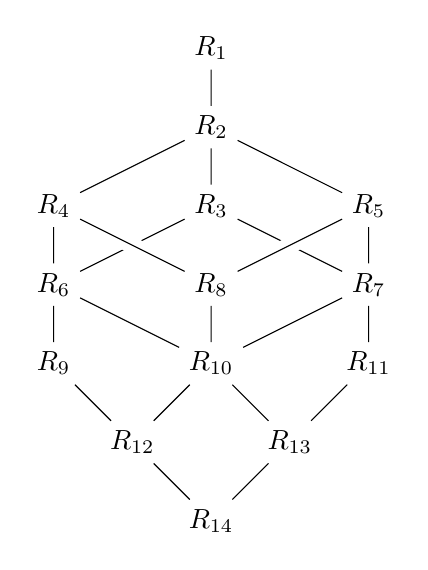
\begin{tikzpicture}
            \node (max) at (0,0) {$R_{14}$};
            \node (12) at (-1,1) {$R_{12}$};
            \node (13) at (1,1) {$R_{13}$};
            \node (9) at (-2,2) {$R_{9}$};
            \node (10) at (0,2) {$R_{10}$};
            \node (11) at (2,2) {$R_{11}$};
            \node (6) at (-2,3) {$R_{6}$};
            \node (8) at (0,3) {$R_{8}$};
            \node (7) at (2,3) {$R_{7}$};
            \node (4) at (-2,4) {$R_{4}$};
            \node (3) at (0,4) {$R_{3}$};
            \node (5) at (2,4) {$R_{5}$};
            \node (2) at (0,5) {$R_{2}$};
            \node (min) at (0,6) {$R_{1}$};
            \draw (min) -- (2) -- (4) -- (6) -- (9) -- (12) -- (max)
            (2) -- (5) -- (7) -- (11) -- (13) -- (max)
            (2) -- (3) -- (6) -- (10) -- (12)
            (3) -- (7) -- (10) -- (13)
            (8) -- (10);
            \draw[preaction={draw=white, -,line width=6pt}] (4) -- (8) -- (5);
        \end{tikzpicture}
    $$
\end{ex}

\subsubsection*{Producto tensorial de \'arboles}
Ahora podemos dar una descripci\'on completa del producto tensorial entre dos objetos representables en $\Omega$ mediante el c\'omputo de su conjunto de shuffles.
\begin{lema}
    Para todo shuffle $R_i$ de $S$ y $T$ tenemos un monomorfismo
    $$
        \xymatrix{
            m\colon\Omega[R_i] \ar@{>->}[r] & \Omega[S]\otimes\Omega[T]
        }
    $$
    El subconjunto dendroidal, que viene dado por la im\'agen de este monomorfismo, lo denotaremos $m(R_i)$.
\end{lema}
\begin{proof}
    Los v\'erties del conjunto dendroidal $\Omega[R_i]$ son las aristas del \'arbol $R_i$. La funci\'on $m$ env\'ia aristas nombradas como $(a,\text{ }x)$ en $R_i$ a la arista con el mismo nombre en $\Omega[S]\otimes\Omega[T]$.
    Vemos que es un monomorfismo.
    No entiendo.
\end{proof}
\begin{corol}
    Para todo objeto $T$ y $S$ en $\Omega$, tenemos que
    $$
        \Omega[S]\otimes\Omega[T] = \bigcup_{i=1}^{N} m(R_i)
    $$
    donde la uni\'on recorre todos los posibles shuffles de $S$ y $T$.
\end{corol}

\subsection{Shuffle de \'arboles en Python}
No es complicado ver que tanto encontrar el producto tensorial de conjuntos dendroidales o, equivalentemente, calcular el conjunto de shuffles para dos \'arboles cualesquiera, resulta una tarea tediosa si los \'arboles son grandes. Para tal problema, el uso de un programa inform\'atico, capaz de almanezar grandes cantidades de informaci\'on al momento de ejecuci\'on, nos resulta c\'omodo, f\'acil y r\'apido.

En este apartado describir\'e de manera breve el c\'odigo que he escrito para poder tratar con op\'eradas, \'arboles, shuffles y finalmente con el conjunto de shuffles. Tambi\'en, el c\'odigo incluye una funci\'on para formar figuras con el paquete \textit{xy} de \textit{Latex} de un \'arbol mediante una descripci\'on b\'asica.

Finalmente, dicho c\'odigo lo podr\'eis encontrar tanto en el Anexo 1 como en el repositorio p\'ublico de c\'odigo de Github: \href{https://github.com/rbrasco/trees-shuffling}{Trees Shuffling}.

\subsubsection*{Clases b\'asicas}
\begin{defi}
    Una \emph{clase inform\'atica} es una abastraci\'on de propiedades y funciones de un objeto en concreto.
\end{defi}

Siguiendo tal definici\'on, tenemos las siguientes clases b\'asicas:
\begin{itemize}
    \item Operada
    \item Arbol
\end{itemize}
Falta por hacer...
\end{document}